\documentclass{article}

\usepackage{fancyhdr}
\usepackage{extramarks}
\usepackage{amsmath}
\usepackage{amsthm}
\usepackage{amsfonts}
\usepackage{tikz}
\usepackage[plain]{algorithm}
\usepackage{algpseudocode}
\usepackage{graphicx}
\usepackage{csquotes}
\usepackage{caption}
\usepackage{subcaption}
\usepackage{hyperref}
\hypersetup{
    colorlinks=true,
    linkcolor=blue,
    filecolor=blue,
    urlcolor=blue
}

\usetikzlibrary{automata,positioning}

%
% Basic Document Settings
%

\topmargin=-0.45in
\evensidemargin=0in
\oddsidemargin=0in
\textwidth=6.5in
\textheight=9.0in
\headsep=0.25in

\linespread{1.1}

\pagestyle{fancy}
\lhead{\hmwkAuthorName}
\chead{\hmwkClass\ (\hmwkClassInstructor): \hmwkTitle}
\rhead{\firstxmark}
\lfoot{\lastxmark}
\cfoot{\thepage}

\renewcommand\headrulewidth{0.4pt}
\renewcommand\footrulewidth{0.4pt}

\setlength\parindent{0pt}

%
% Create Problem Sections
%

\newcommand{\enterProblemHeader}[1]{
    \nobreak\extramarks{}{Problem \arabic{#1} continued on next page\ldots}\nobreak{}
    \nobreak\extramarks{Problem \arabic{#1} (continued)}{Problem \arabic{#1} continued on next page\ldots}\nobreak{}
}

\newcommand{\exitProblemHeader}[1]{
    \nobreak\extramarks{Problem \arabic{#1} (continued)}{Problem \arabic{#1} continued on next page\ldots}\nobreak{}
    \stepcounter{#1}
    \nobreak\extramarks{Problem \arabic{#1}}{}\nobreak{}
}

\setcounter{secnumdepth}{0}
\newcounter{partCounter}
\newcounter{homeworkProblemCounter}
\setcounter{homeworkProblemCounter}{1}
\nobreak\extramarks{Problem \arabic{homeworkProblemCounter}}{}\nobreak{}

%
% Homework Problem Environment
%
% This environment takes an optional argument. When given, it will adjust the
% problem counter. This is useful for when the problems given for your
% assignment aren't sequential. See the last 3 problems of this template for an
% example.
%
\newenvironment{homeworkProblem}[1][-1]{
    \ifnum#1>0
        \setcounter{homeworkProblemCounter}{#1}
    \fi
    \section{Problem \arabic{homeworkProblemCounter}}
    \setcounter{partCounter}{1}
    \enterProblemHeader{homeworkProblemCounter}
}{
    \exitProblemHeader{homeworkProblemCounter}
}

%
% Homework Details
%   - Title
%   - Due date
%   - Class
%   - Section/Time
%   - Instructor
%   - Author
%

\newcommand{\hmwkTitle}{Assignment\ \#5}
\newcommand{\hmwkDueDate}{November 17, 2020}
\newcommand{\hmwkClass}{SCI 238}
\newcommand{\hmwkClassInstructor}{Dr. Michael Fich}
\newcommand{\hmwkAuthorName}{\textbf{Zach Bortoff}}

%
% Title Page
%

\title{
    \vspace{2in}
    \textmd{\textbf{\hmwkClass:\ \hmwkTitle}}\\
    \normalsize\vspace{0.1in}\small{Due\ on\ \hmwkDueDate\ at 11:59pm}\\
    \vspace{0.1in}\large{\textit{\hmwkClassInstructor}}
    \vspace{3in}
}

\author{\hmwkAuthorName}
\date{}

\renewcommand{\part}[1]{\textbf{\large Part \Alph{partCounter}}\stepcounter{partCounter}\\}

%
% Various Helper Commands
%

% Useful for algorithms
\newcommand{\alg}[1]{\textsc{\bfseries \footnotesize #1}}

% For derivatives
\newcommand{\deriv}[1]{\frac{\mathrm{d}}{\mathrm{d}x} (#1)}

% For partial derivatives
\newcommand{\pderiv}[2]{\frac{\partial}{\partial #1} (#2)}

% Integral dx
\newcommand{\dx}{\mathrm{d}x}

% Alias for the Solution section header
\newcommand{\solution}{\textbf{\large Solution}}

% Probability commands: Expectation, Variance, Covariance, Bias
\newcommand{\E}{\mathrm{E}}
\newcommand{\Var}{\mathrm{Var}}
\newcommand{\Cov}{\mathrm{Cov}}
\newcommand{\Bias}{\mathrm{Bias}}

\begin{document}

\maketitle

\pagebreak

\begin{homeworkProblem}
	\textbf{Estimate the number of Solar neutrinos passing through a detector on the
Earth in one second.} Assume that the detector has a surface area of 1.0 square
meters and is aligned so that it faces directly towards the centre of the Sun.
Assume that every neutrino travels without any change (i.e. none are absorbed or
converted to a different particle). Also assume that the energy carried out of the
Sun by the neutrinos is negligible. As always, show your calculations. (Marks: 4)
\textit{Warning: This is discussed in the textbook… But it gives the wrong numbers –
don’t worry if your calculation does not produce those numbers in the text!}\\

    \textbf{Solution}

	Let \(t = 1 \hspace{3pt}[s]\) denote the period over which neutrinos are being measured, \(A_{detec} = 1\hspace{3pt} [m]\) denote the area of the detector, and \(E_{p-p}\) denote the energy released by 1 proton-proton chain reaction.\\
	
	First, we need to determine the value of \(E_{p-p}\). According to the book, the mass difference created by one proton-proton chain reaction is \(\sim 0.02862 \hspace{3pt} [u]\). By applying the mass-energy equivalence equation, we can obtain the energy of one proton-proton chain reaction: \(E_{p-p}=m_{p-p}c^2=(0.02862 \hspace{3pt}[u]) (3\times 10^8 \hspace{3pt} [m/s]) \approx 26.696 \hspace{3pt} [MeV]\).\\
	
	Now, the energy released by the Sun over a period of \(t\) seconds is \(E_{Sun}=L_{Sun} t=(3.846\times 10^{26} \hspace{3pt}[W]) (1 \hspace{3pt} [s]) = 3.846\times 10^{26} [J]\).\\
	
	Assuming that the only things contributing to the Sun's luminosity are the proton-proton chain reactions, we can infer that the number of proton-proton chains required to produce \(E_{Sun}\) is: \(n_{reaction}=E_{Sun}/E_{p-p}\approx8.99\times10^{37} \hspace{3pt} [reactions]\). \\
	
	We know that the proton-proton chain releases \(2\) neutrinos, so the total number of neutrinos released per second by the Sun is: \(N_{neutrino}=2n_{reaction}\approx1.80\times10^{38} \hspace{3pt} [neutrinos]\).\\
	
	Assuming that the neutrinos do not react with anything and that they are released uniformly in each direction, then the density of neutrinos \([neutrino/m^2]\) projected on an imaginary sphere \(1 \hspace{3pt} [AU]\) around the center of the Sun would be \(\rho_{neutrino}=N_{neutrino} / 4\pi r^2\approx6.39\times 10^{14} \hspace{3pt} [neutrinos/m^2]\). \\
	
	There is a detector with an area of \(A_{detect}\) on that imaginary sphere measuring the flux of neutrinos. The number of neutrinos passing through that detector every second is \(\rho_{neutrino} A_{detect} = 6.39\times 10^{14} \hspace{3pt} [neutrinos]\).
	

\end{homeworkProblem}

\pagebreak


\begin{homeworkProblem}
 	2) (a) Plot, on a log-log scale, the Main Sequence lifetime versus Mass for the
star types shown on the table below. Do this two ways: approximating the
lifetime using the observed mass and luminosity (from the table below, and as
discussed in Lecture) and using the results of theoretical models (also shown in
the table below). (b) Draw a line on the plot in (a) for the mass-dependent (only)
mathematical approximation shown in class. (It gives the lifetime after making a
simplifying assumption about luminosity to produce a lifetime estimate that is
based only on the mass.) (c) Discuss these three sets of results for the lifetime.
(Marks: 6) \textit{Assume that the lifetime of the Sun exactly 1010 years for the two
approximations.} \\
 	
 	\textbf{Solution}
 	
 	(a/b.)
 	
 	\begin{figure}[!h]
       	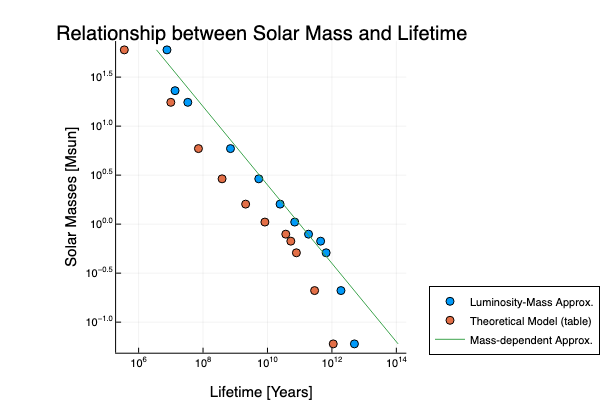
\includegraphics[width=0.95\textwidth]{SolarMassLifetime.png}
        	\centering
    		\caption{Log-log plot of predicted lifetime to solar mass (made diagram with Julia)}
    		\label{fig:Earth}
    	\end{figure}
    	Example Calculations:\\
    	Luminosity-Mass Approximation:
    	\[
    		\tau_1 = 10^{10} \frac{M_1}{L_1} = 10^{10} \frac{60}{3.6\times 10^{5}}\approx 7.59 \times 10^{6}
    	\]\\
    	
    	Mass-dependent Approximation:\\
    	\[
    		\tau_1 = 10^{10} (\frac{1}{M_1})^{2.5} = 10^{10} \frac{1}{3.6\times 10^{5}}\approx 3.59 \times 10^{6}
    	\]\\
 	
 	(c.) The overall trend of both heuristic approaches matches the overall trend of the model - which we can take to be the gold standard here. This trend is characterized by a more or less constant, negative slope starting near \((10^6, 10^{1.5})\) and ending near \((10^{13}, 10^{-1.0})\).  \\
 	
 	The slopes of both the Luminosity-Mass approximation and the model prediction become more negative at lower Solar Masses, deviating ever more from the Mass-dependent approximation line. This suggests that some  assumption undergirding the Mass-dependent approximation may be getting violated at lower Solar masses, rendering that heuristic less accurate. One such assumption could be that the \(L \propto M^{3.5}\), which would make sense, because that is this assumption after all that transforms the Luminosity-Mass approximation (which seems generally just as accurate at lower Solar Masses as it is at other Solar Masses) to the final form of the Mass-dependent approximation. Indeed, a more general form of the Mass-luminosity relation than the form studied in class breaks down the exponent on the Mass term into different values based on the star's mass range [\href{https://jila.colorado.edu/~pja/astr3730/lecture18.pdf}1].  \\
 	
 	Another interesting characteristic of the plot is that the model's predictions of lifetime are consistently smaller than those of both the Luminosity-Mass approximation and the Mass-dependent approximation. Perhaps this is because the heuristic approaches neglect to multiply by some constants, which in a log-log plot would manifest in the form of a vertical translation. \\

 	
	
\end{homeworkProblem}

\pagebreak

\end{document}
